\documentclass[../main.tex]{subfiles}

\begin{document}
	\subsection{The Principle Of Least Privilege}
	As previously stated the principle of least privilege (PoLP) requires that components of a system operate with the minimum resources required to complete their respective tasks. PoLP is heavily utilized in systems security research to design systems that maintain their integrity in the face of an adversary capable of exploiting some of their components. In contrast, the most popular web servers today execute as monolithic applications, including Apache and NGINX, where all of their processes have the same level of privilege and have access to the sensitive key material. Exploiting any one of these processes may therefore lead to leaking the private key. 

	To motivate the design of our system, we begin by discussing a system called Wedge~\cite{Bittau08} that was used to refactor Apache, by enforcing PoLP, securing the private key in the face of an adversary who is capable of exploiting the web server application. First, we list the attacks possible against a monolithic web server and then detail how the design implemented with Wedge resolved these vulnerabilities. 

	\paragraph{Possible Attacks} There are two main types of attacks that may be mounted by an adversary capable of exploiting \textit{only} the network facing component of the web server application:
	\begin{enumerate}
		\item The adversary could leak the private key from the network facing component, which has to run as root to bind to port 80. This could be by reading the private key from disk directly or from the process's memory space. The attack is illustrated in Figure~\ref{fig:attack1}.

		\begin{figure}[H]
			\centering
			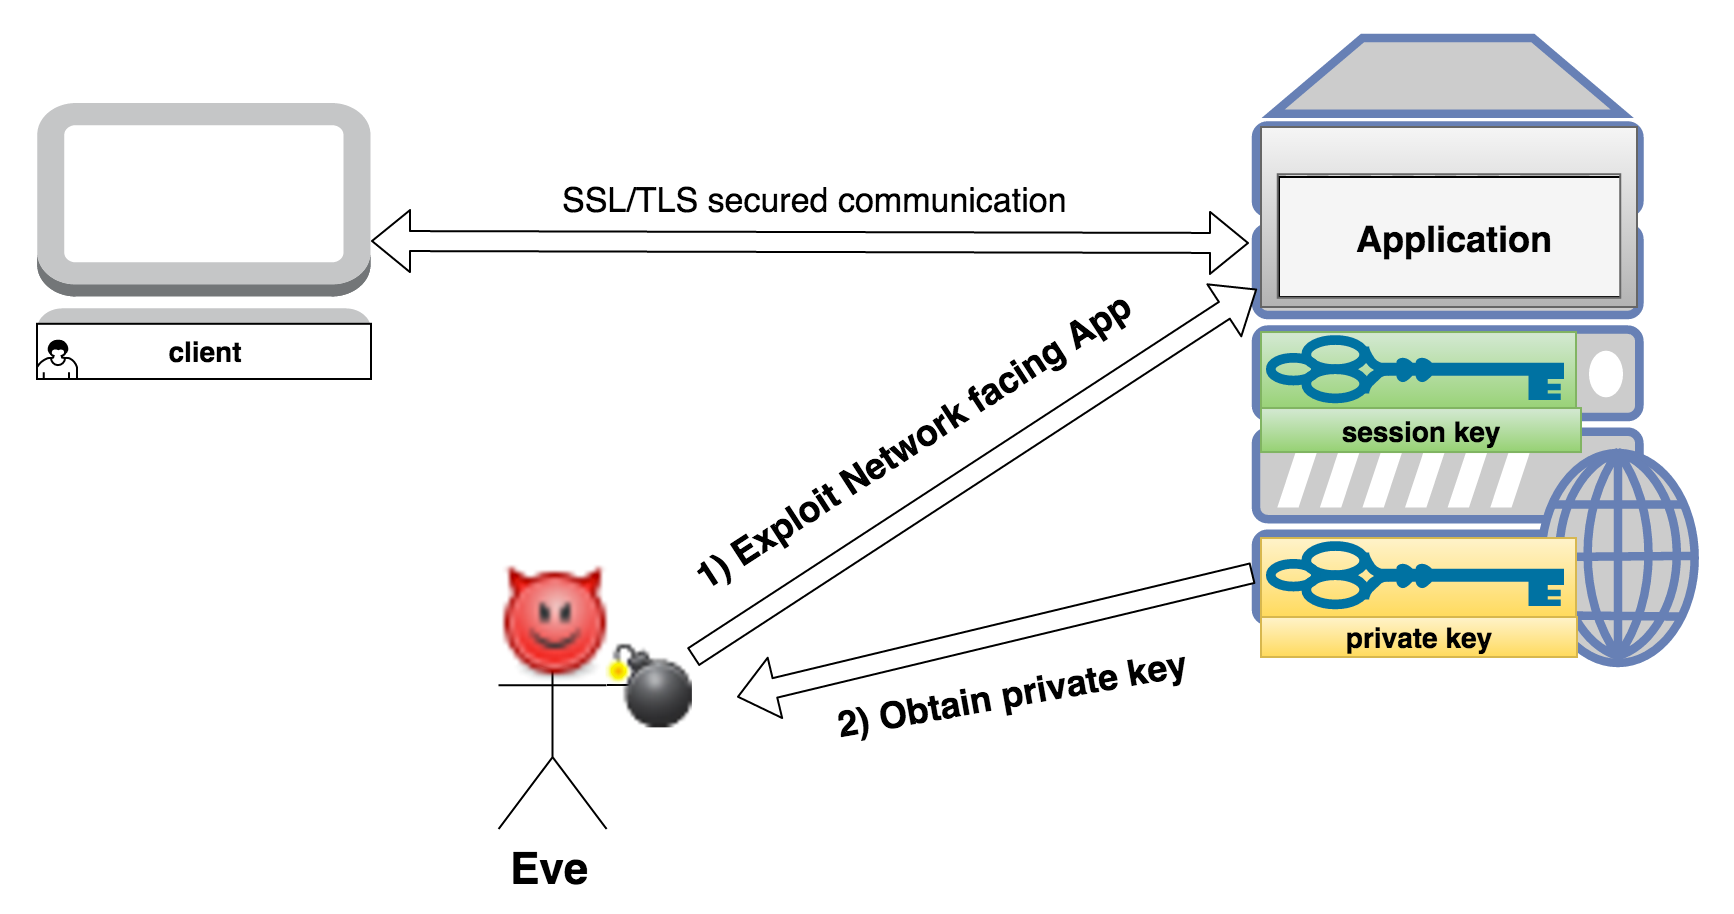
\includegraphics[scale=0.15]{images/attack1.png}
			\label{fig:attack1}
			\caption{Exploiting the network facing component to leak the private key}
		\end{figure}

		%add a foot note explaining the naive session key generation
		\item The adversary may record traffic exchanged over the SSL/TLS channel and then exploit a naive session key generation interface to acquire the session keys used in that exchange. This exploit only works if the cipher used is one that does not offer perfect forward secrecy (PFS). The session key generation operations require use of the private key, but the adversary does not need to learn the key to complete this attack. However, this attack only affects the single session which was eavesdropped. The attack is illustrated in Figure~\ref{fig:attack2}.

		\begin{figure}[H]
			\centering
			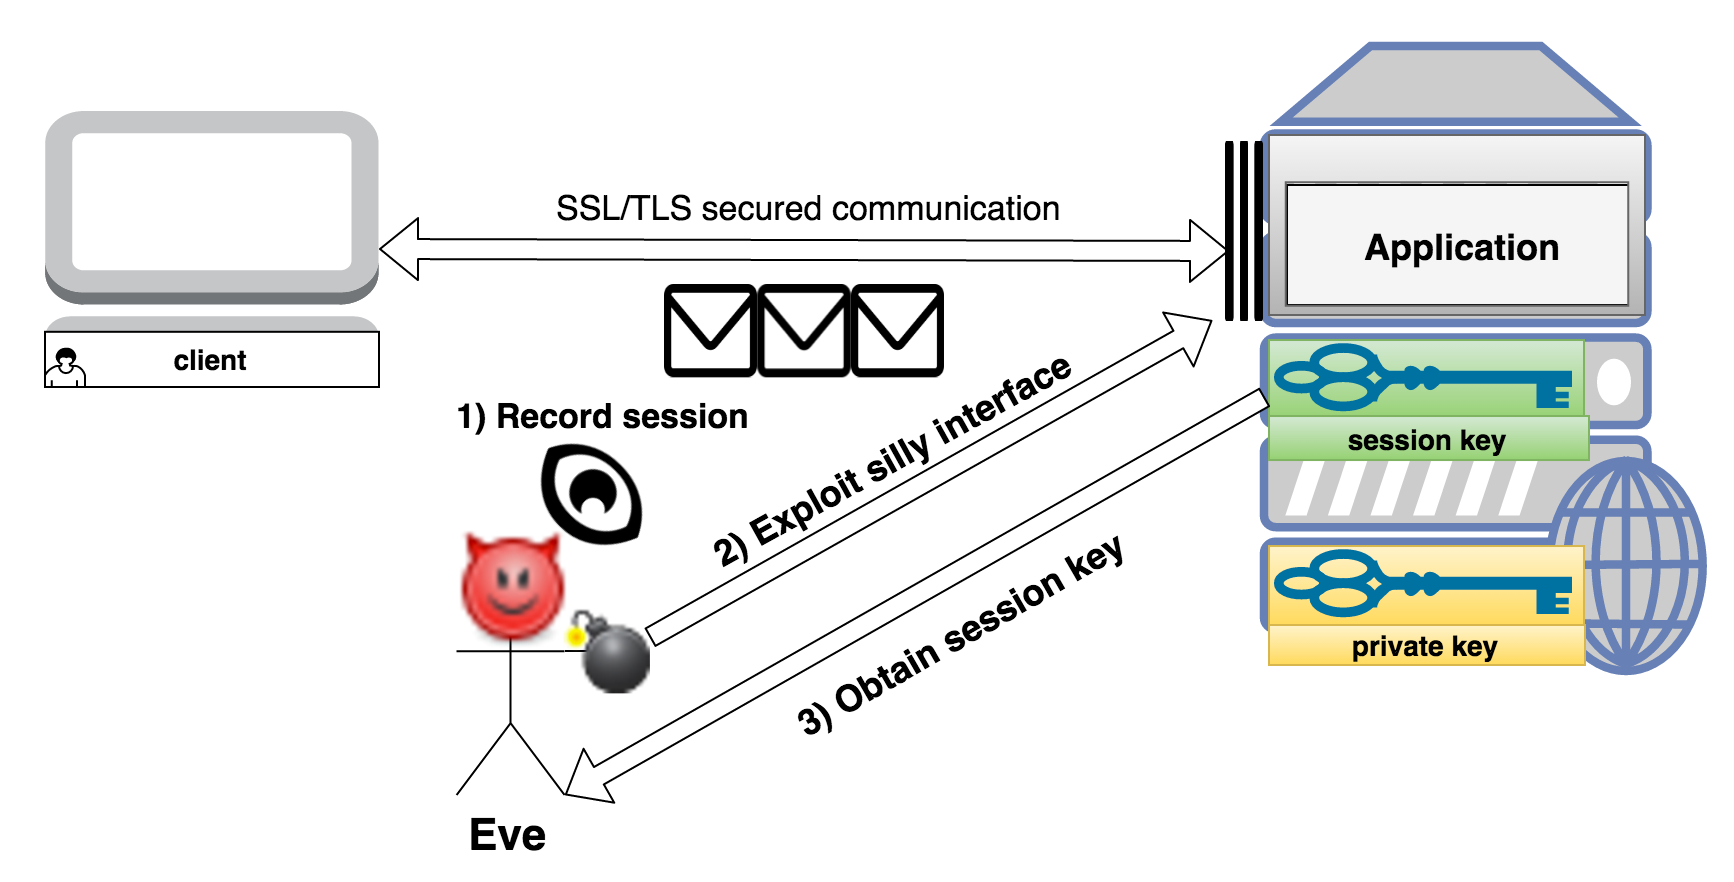
\includegraphics[scale=0.15]{images/attack2.png}
			\label{fig:attack2}
			\caption{Exploiting the network facing component and the naive session key generation interface to generate session keys for eavesdropped session}
		\end{figure}
	\end{enumerate}

\end{document}